\documentclass[12pt]{standalone}

% tikz
\usepackage{lmodern}                                       % solve font issue
\usepackage[T1]{fontenc}

\usepackage{tikz}
\usepackage{pgfplots}

\usetikzlibrary{arrows}
\usepgfplotslibrary{fillbetween}                           % LaTeX and plain TeX
\pgfplotsset{width=203pt,height=203pt,compat=1.15}         % compatibility for PGFPlots 1.15


% color
\definecolor{zzttqq}{rgb}{0.6,0.2,0}
\definecolor{xdxdff}{rgb}{0.49,0.49,1}
\definecolor{ududff}{rgb}{0.3,0.3,1}
\definecolor{qqwuqq}{rgb}{0,0.39,0}
\definecolor{cqcqcq}{rgb}{0.75,0.75,0.75}

\begin{document}
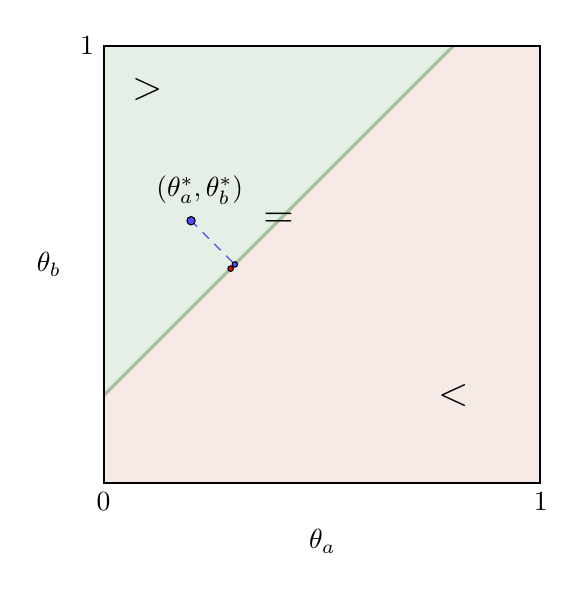
\begin{tikzpicture}[line cap=round, line join=round, >=triangle 45]
	\begin{axis} [
			xmin=0,xmax=1,xtick={1},xtick style={draw=none},
			ymin=0,ymax=1,ytick={1},ytick style={draw=none},
			extra x ticks={0},
			xlabel=$\theta_a$, ylabel=$\theta_b$, ylabel style={rotate=-90},
			axis equal=true,
			enlargelimits=false,
		]

		\addplot[opacity=0.3, line width=1.2pt, color=qqwuqq, smooth, samples=5, domain=0:1-0.2] {x + 0.2};

		% Filled region
		\fill [domain=0:1, variable=\x, fill=qqwuqq, fill opacity=0.1, smooth, samples=5]
		(0,0.2) -- plot (\x,{\x+0.2}) -- (1-0.2,1) -- (0,1) -- cycle;

		% Filled region
		\fill [domain=0:1, variable=\x, fill=zzttqq, fill opacity=0.1, smooth, samples=5]
		(0,0) -- (0,0.2) --
		plot (\x,{\x+0.2}) -- (1-0.2,1) -- (1,1) -- (1,0) -- cycle;

		% Dashed diagonal line
		\draw [line width=0.5pt, color=ududff, opacity=0.9, dashed] (0.2,0.6) -- (0.3,0.5);


		% Rectangle borders
		\draw [line width=1pt, color=black] (0,0) -- (0,1);
		\draw [line width=1pt, color=black] (1,1) -- (1,0);
		\draw [line width=1pt, color=black] (1,0) -- (0,0);
		\draw [line width=1pt, color=black] (0,1) -- (1,1);

		% Labels
		\begin{scriptsize}
			\draw (0.1,0.9) node {\bf \Large $>$};

			\draw (0.4,0.6) node {\Large $=$};

			\draw (0.8,0.2) node {\Large $<$};

			\draw (0.22,0.67) node {$(\theta_a^*, \theta_b^*)$};

			\draw [fill=red] (0.2904,0.4904) circle (1pt);

			\draw [fill=ududff] (0.3,0.5) circle (1pt);
			% Points with original comments
			\draw [fill=ududff] (0.2,0.6) circle (1.5pt);

		\end{scriptsize}
	\end{axis}
\end{tikzpicture}
\end{document}